\documentclass[fontsize=11pt]{article}
\usepackage{amsmath}
\usepackage{soul}
\usepackage{graphicx}
\usepackage[utf8]{inputenc}
\usepackage[margin=0.75in]{geometry}
\graphicspath{ {pics/} }

% Commands
\newcommand{\ttt}[1]{\texttt{#1}}

\title{CSC111 Project Report: COVID-19 Contact Visualization}
\author{Patricia Ding, Salman Husainie, Simon Chen, Makayla Duffus}
\date{\today}

\begin{document}
    \maketitle

    \section*{Problem Description and Research Question}
    The effect of COVID-19 on individuals at an international level is well-known and indubitable due to broadcasts almost daily in the public news. While the immediate impacts on one's personal life may be visible, the general behaviour and impact on similarly sized communities are out of sight and reach. Contact tracing, a process employed by the government to slow the spread of the virus, identifies those possibly at risk of contracting the virus and guides self-isolation (WHO). The possibility that one may get severely ill from COVID-19 is directly affected by their pre-existing medical conditions. For example, individuals dealing with cancer, heart conditions, and obesity are at a higher risk of hospitalization due to COVID-19 (CDC). Also, individual susceptibility is impacted by social attitudes such as whether the community follows the government's instruction for social distancing and the use of personal protective equipment. Research suggests that proper and widespread use of face coverings reduces the risk of infection by 65 percent (UCDAVIS). Furthermore, the severity of the infection can lead to a patient developing complicating health conditions such as severe organ damage in the heart, lungs, and/or brain (Mayo Clinic). Once contracted, the severity of the illness is dependant on the following factors: age, sex, viral strain, ethnic background, underlying health conditions and gaps in one's immune system, etc. (Weill Cornell Medicine).\\
    \newline
    \noindent
    Our concern is how COVID-19 spreads on the community level. It is in analyzing these smaller communities that we gain a greater understanding of spreads for national and global level trends. While the importance of collecting and analyzing data on a national and global level remains for economic and societal reasons, in order to completely understand any complex problem, we must investigate at the smallest level. Government contact tracing does not go as deep (level-wise) as we are interested in and they do not account for the impact possible underlying medical conditions have on the potentiality of people becoming infected (COVID-19 contact tracers). The problem we are interested in answering is: \textbf{How can we create an interactive visualization of the spread of COVID-19 in communities/friend groups?}
    \newpage
%
    \section*{Datasets}
    There are two main types of datasets used in this program: the randomly generated graphs created by our program, and the two csv files we extract data from.\\
    \newline
    \textbf{Randomly Generated Graphs}\\
    \newline
    The data generated from within the program, stored in a Graph object, represents a varied community size (dependant on user input from 10 to 60 members), with a specified connectivity level and involves general contact randomness. The Graph object being generated consists of vertices of a new class, \_Person, with the respective attributes, and contains weighted edges with the level of contact between two objects (people) as the weight. Moreover, the randomly generated graphs can be connected or disconnected depending on the user's specification.\\
    \newline
    \textbf{CSV Files}\\
    The provided CSV files are self-made, together representing a sample community that consists of ten members. These ten members create a disconnected graph with twelve edges and random levels of contact.\\
    \newline
    While the two CSV files are pre-made, to increase the scope of this project, it was decided that the user is given permission to modify the content of these files. By adding or removing whole lines of either file, the user is able to create their own community to be represented in a Graph object. As long as the formatting of each file is preserved and the required fields, (as outlined in the first line of each file) are filled, the program will be able to perform with the given files. Furthermore, because the CSV files are pre-made, they are optimized so that every column and row is used by the program. In other words, every variable in the CSV file is used to create the sample community.\\
    \newline
    \ttt{persons.csv} \\
    This pre-made file in CSV format is to be used in unison with the connections.csv file to represent a small community of 10 members (as previously described). The data in this file represents information that will be used to create a \_Person object. Each row contains an arbitrary person's 6 digit identifier (for real life privacy purposes), first and last name, age, and severity level if they were to contract COVID-19. Each attribute (id, name, age, severity) has restrictions on what counts as a valid input. The id must be a string of size 6 with any combination of uppercase and integer values so long as the identifiers are unique. This uniqueness also applies to the names, no two names can be the same. The names have no length or content restriction. The age must lie between numbers 18 and 55, inclusive. The severity is a decimal(float value) representing the percentage of severity where 1.0 is the highest, and 0.0 the lowest.\\
    \begin{figure}[h]
        \centering
        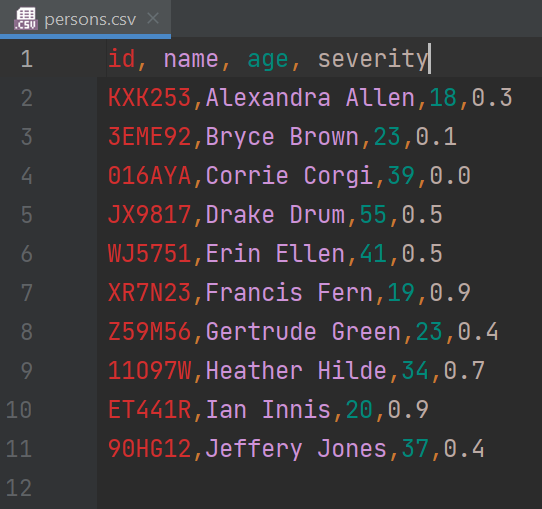
\includegraphics[width=60mm,scale=0.3]{pictures/person_dataset.png}
        \caption{Person Dataset}
    \end{figure}
    \newpage
    \section*{Datasets Continued}
    \ttt{connections.csv} \\
    As mentioned above, this pre-made file in CSV format is to be used with \ttt{persons.csv} file to generate a sample small community graph. The data in this file will be used create edges between each \_Person object in the main graph object. Each row contains the two unique identifiers (each corresponding to separate identifiers in \ttt{persons.csv}), and a decimal from 0.05 to 1.0 that represents the level of contact between the two individuals (where 1.0 is the highest level of contact). Furthermore, the randomly generated graphs can be specified to be either disconnected or connected.

    \begin{figure}[h]
        \centering
        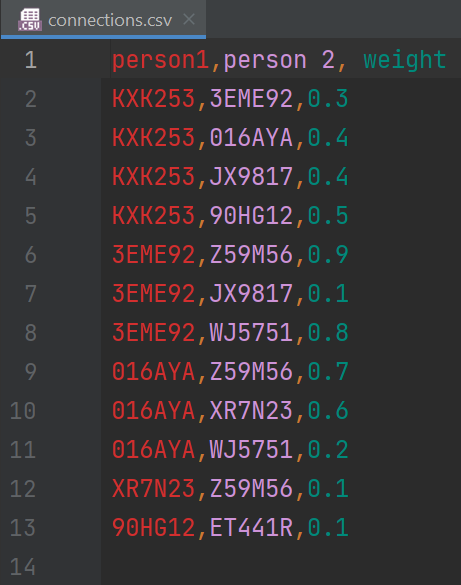
\includegraphics[width=60mm,scale=0.3]{pictures/connections_dataset.png}
        \caption{Connection Dataset}
    \end{figure}


    \newpage
    \section*{Computational Overview}
    \textbf{Data Classes}\\
    There are three main classes used in this project: \ttt{\_Person}, \ttt{Graph}, and \ttt{Simulation}.\\
    \newline
    The \ttt{\_Person} data class represents an individual in a social network. In other words, this object represents a vertex in the \ttt{Graph} data class described later. They have the following attributes and types: a unique identifier(str), unique name(str), their age(int), severity level(float), neighbours with corresponding contact levels(dict[\_Person, float]), and their degree separation from an infected person(int). The most important method within this data class, \ttt{calculate\_degrees\_apart()}, updates the degrees\_apart attribute of the \_Person and their neighbours so that the initial \ttt{\_Person} object's \ttt{degrees\_apart} attribute is the smallest possible value. \\
    \newline
    \noindent
    The \ttt{Graph} data class is the main structure within the program. It represents a community of \ttt{\_Person} objects. It has one attribute, \ttt{\_people}, a dictionary which maps the unique identifier to its respective \ttt{\_Person} object. The methods of the \ttt{Graph} function can be separated into three categories: accessor methods, mutation methods, and \ttt{NetworkX} conversion methods. The accessor methods return certain values from the \ttt{\_people} attribute that are used to create the simulation. The mutation methods are used to add vertices/edges, and recalculate the degrees\_apart attribute of the \ttt{\_Person} objects contained within the graph. As the name implies, the \ttt{NetworkX} conversion methods allows us to convert our \ttt{Graph} data class into a \ttt{NetworkX} graph that can be used to visualize later in the simulation.\\
    \newline
    \noindent
    The \ttt{Simulation} data class is described later in the computational overview.\\
    \newline
    \noindent
    \textbf{GUI Menu}\\
    When the user runs the program, they are met with a user interface that allows them to generate a social network of individuals through a graph consisting of \ttt{\_Person} objects. This user interface is created with two modules: \ttt{pygame}, and \ttt{pygame\_gui}. The Python module used to create this is \ttt{menu.py}.\\
    \newline
    \textbf{Graph Generation}\\
    Generating graphs for the simulation can be done in one of two ways: loading the data from a CSV file, or creating a randomly generated connected (or disconnected) graph.\\
    \newline
    The former is done through the function \ttt{load\_graph\_csv}. The function adds vertices to the graph through the \ttt{names\_files} parameter, and then adds weighted edges from the data within \ttt{contact\_file}.\\
    \newline
    The latter, creating a random connected (or disconnected) graph is done through the \ttt{generate\_connected\_graph} function. This function returns a connected graph with a specified number of \_Person objects and connectivity level. Through the use of helper functions, attributes for each \ttt{\_Person} object (i.e. identifier, name, edge weight) are randomly generated and added to the graph. Edges are then made between \ttt{\_Person} objects to create a connected graph. The weight between edges are randomly selected from a range determined by a parameter given by the user (connectivity level). \\
    \newline
    The generation of a disconnected graph follows a similar algorithm to the generation of a connected graph. Given the number of desired nodes, it separates a small fraction of these nodes, calls \ttt{generate\_connected\_graph} with the larger portion, and then with this returned graph, the function randomly creates and adds edges between \ttt{\_Person} objects from the group that was initially separated.\\
    \newline
    \noindent
    \textbf{Using \ttt{networkx}} \\
    In order to display our graphs, we use the \ttt{networkx} library similar to Assignment 3. The core difference is when loading converting our graphs from \ttt{social\_graph.Graph} to a networkx graph (using the \ttt{social\_graph.Graph.to\_nx()} (and similar) methods, which ensure that the networkx nodes have a proper colour by adding a node attribute "colour" that is calculated based off of either the simulation colours, or the degree visualization colours in the \ttt{colouring} module.
    \newpage
    \section*{Computational Overview Continued}
    \textbf{Degree Calculation} \\
    The degree calculation works similar to the depth first search algorithm we learned in class. When we want to display the degrees apart from an infected person for each node, we first set every node's \ttt{degrees\_apart} attribute to \ttt{None}. Then, for every infected node, we first set \ttt{degrees\_apart} to 0, then we call the recursive method \ttt{Person.calculate\_degrees\_apart()} which changes the neighbour's \ttt{degrees\_apart} attribute to be an additional +1 degrees apart from the current node. This recurses until all connected nodes are calculated. To ensure that \ttt{degrees\_apart} is representative of the minimum distance between the person and an infected person, upon setting \ttt{degrees\_apart} for that person, we make sure that the current \ttt{degrees\_apart} isn't already less than the one we want to set. In those cases, we leave it as the minimum. \\ \\
    After everything runs smoothly, we then compute the colours based off of the \ttt{degrees\_apart} attribute of each node, modelled after an exponential decay function in the \ttt{colouring} module, then open theuplotly graph for the user to see.
    \\ \\
    \textbf{How does the simulation work?} \\
    The simulation method shown in CSC110 was an event-based food delivery system.Having an event queue of events to handle, does not have a discrete interval of time between events. If you wanted to show what the simulation looked like every week (rather than every time someone got infected), you would think of using a \emph{tick-based} model, where a \emph{tick} a discrete unit of time between moments in a simulation. In our \ttt{simulation.Simulation} class, we say a tick is equivalent to one week.
    \\ \\
    We start by loading an initial state of our simulation into the class, which stores an instance of a \ttt{social\_graph.Graph} with all its data. Each tick, we calculate using values like edge weights (closeness between individuals) and randomly generated values to determine whether or not a given neighbour to an infected person will be infected on the next tick. If they are chosen to be infected on the next tick, they will be added to a buffer which, at the start of every new tick, sets all the people inside to be infected, then clears its values. Every tick, the state of the \ttt{social\_graph.Graph} gets converted into a \ttt{networkx} graph, and is kept track of and stored into a \ttt{plotly.graph\_objects.Frame}, which is a \ttt{plotly} class that stores all the data of the graph at a given tick. Once the simulation has gone through the full 21 ticks (21 weeks), the frames are then rendered using the \ttt{visualization.render\_simulation\_full()} function, which takes all the frames and generates a plotly web-display of the graph, similar to Assignment 3. This display however, comes with a few very powerful simulation-specific features: The timeline slider, the play-button, and a dynamic title.
    \newpage
    \section*{Instructions}
    After installing the necessary libraries listed in the requirements.txt file, the two optional datasets can be found on UTSend (Claim ID: kS3VcPBFWTvqNF72 with Claim Passcode: Bcrrvrb55Cb5dPVR). While our program does not require the given datasets to operate, as this is an additional feature, if the user desires to use these files, the 2 datasets should be placed onto a folder named ‘data’ that exists in the same space as the remaining program files (main.py, simulation.py, ...). In other words, the sub-folder ‘data’ is in the same folder as the other program files. To generate results using these CSV files, code can be executed in the console using modified inputs to the functions in main.py. \\
    \noindent
    Upon running the \ttt{main.py} module, the user will be greeted with an interactive menu that allows them to set different properties of the simulated social network. The first condition determines how many people are in the simulation. "Level of Closeness" determines how likely a non-infected individual can contract COVID-19. The last two conditions are self-explanatory. For example, the conditions shown below would generate a connected graph simulation consisting of 20 people with "medium" level closeness, and one infected person.
    \begin{figure}[h]
        \centering
        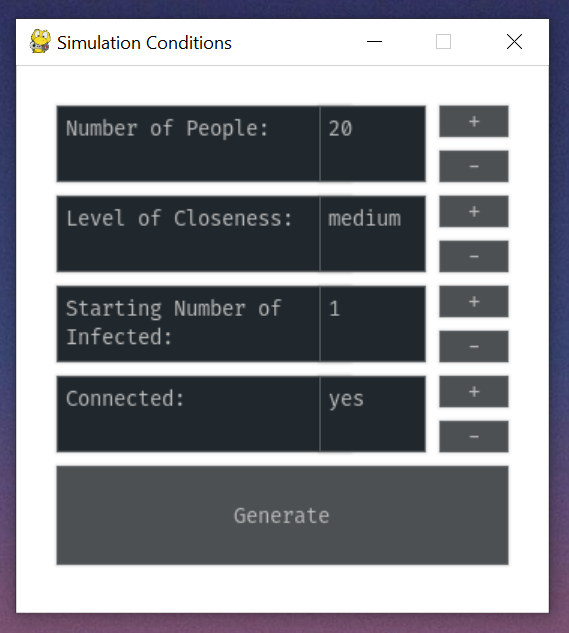
\includegraphics[width=45mm,scale=0.3]{pictures/gui_menu.png}
        \caption{The GUI User Menu}
    \end{figure}
    \newline
    Besides the GUI menu, there are a variety of different runner functions in the \ttt{main.py} module. These runners are split into two categories: CSV runners, and generated graph runners. To test them, simply call them within the main block. For example, upon calling the runner \ttt{run\_simulation\_csv} with the appropriate parameters, the user will be presented with the following screen on their web browser:
    \begin{figure}[h]
        \centering
        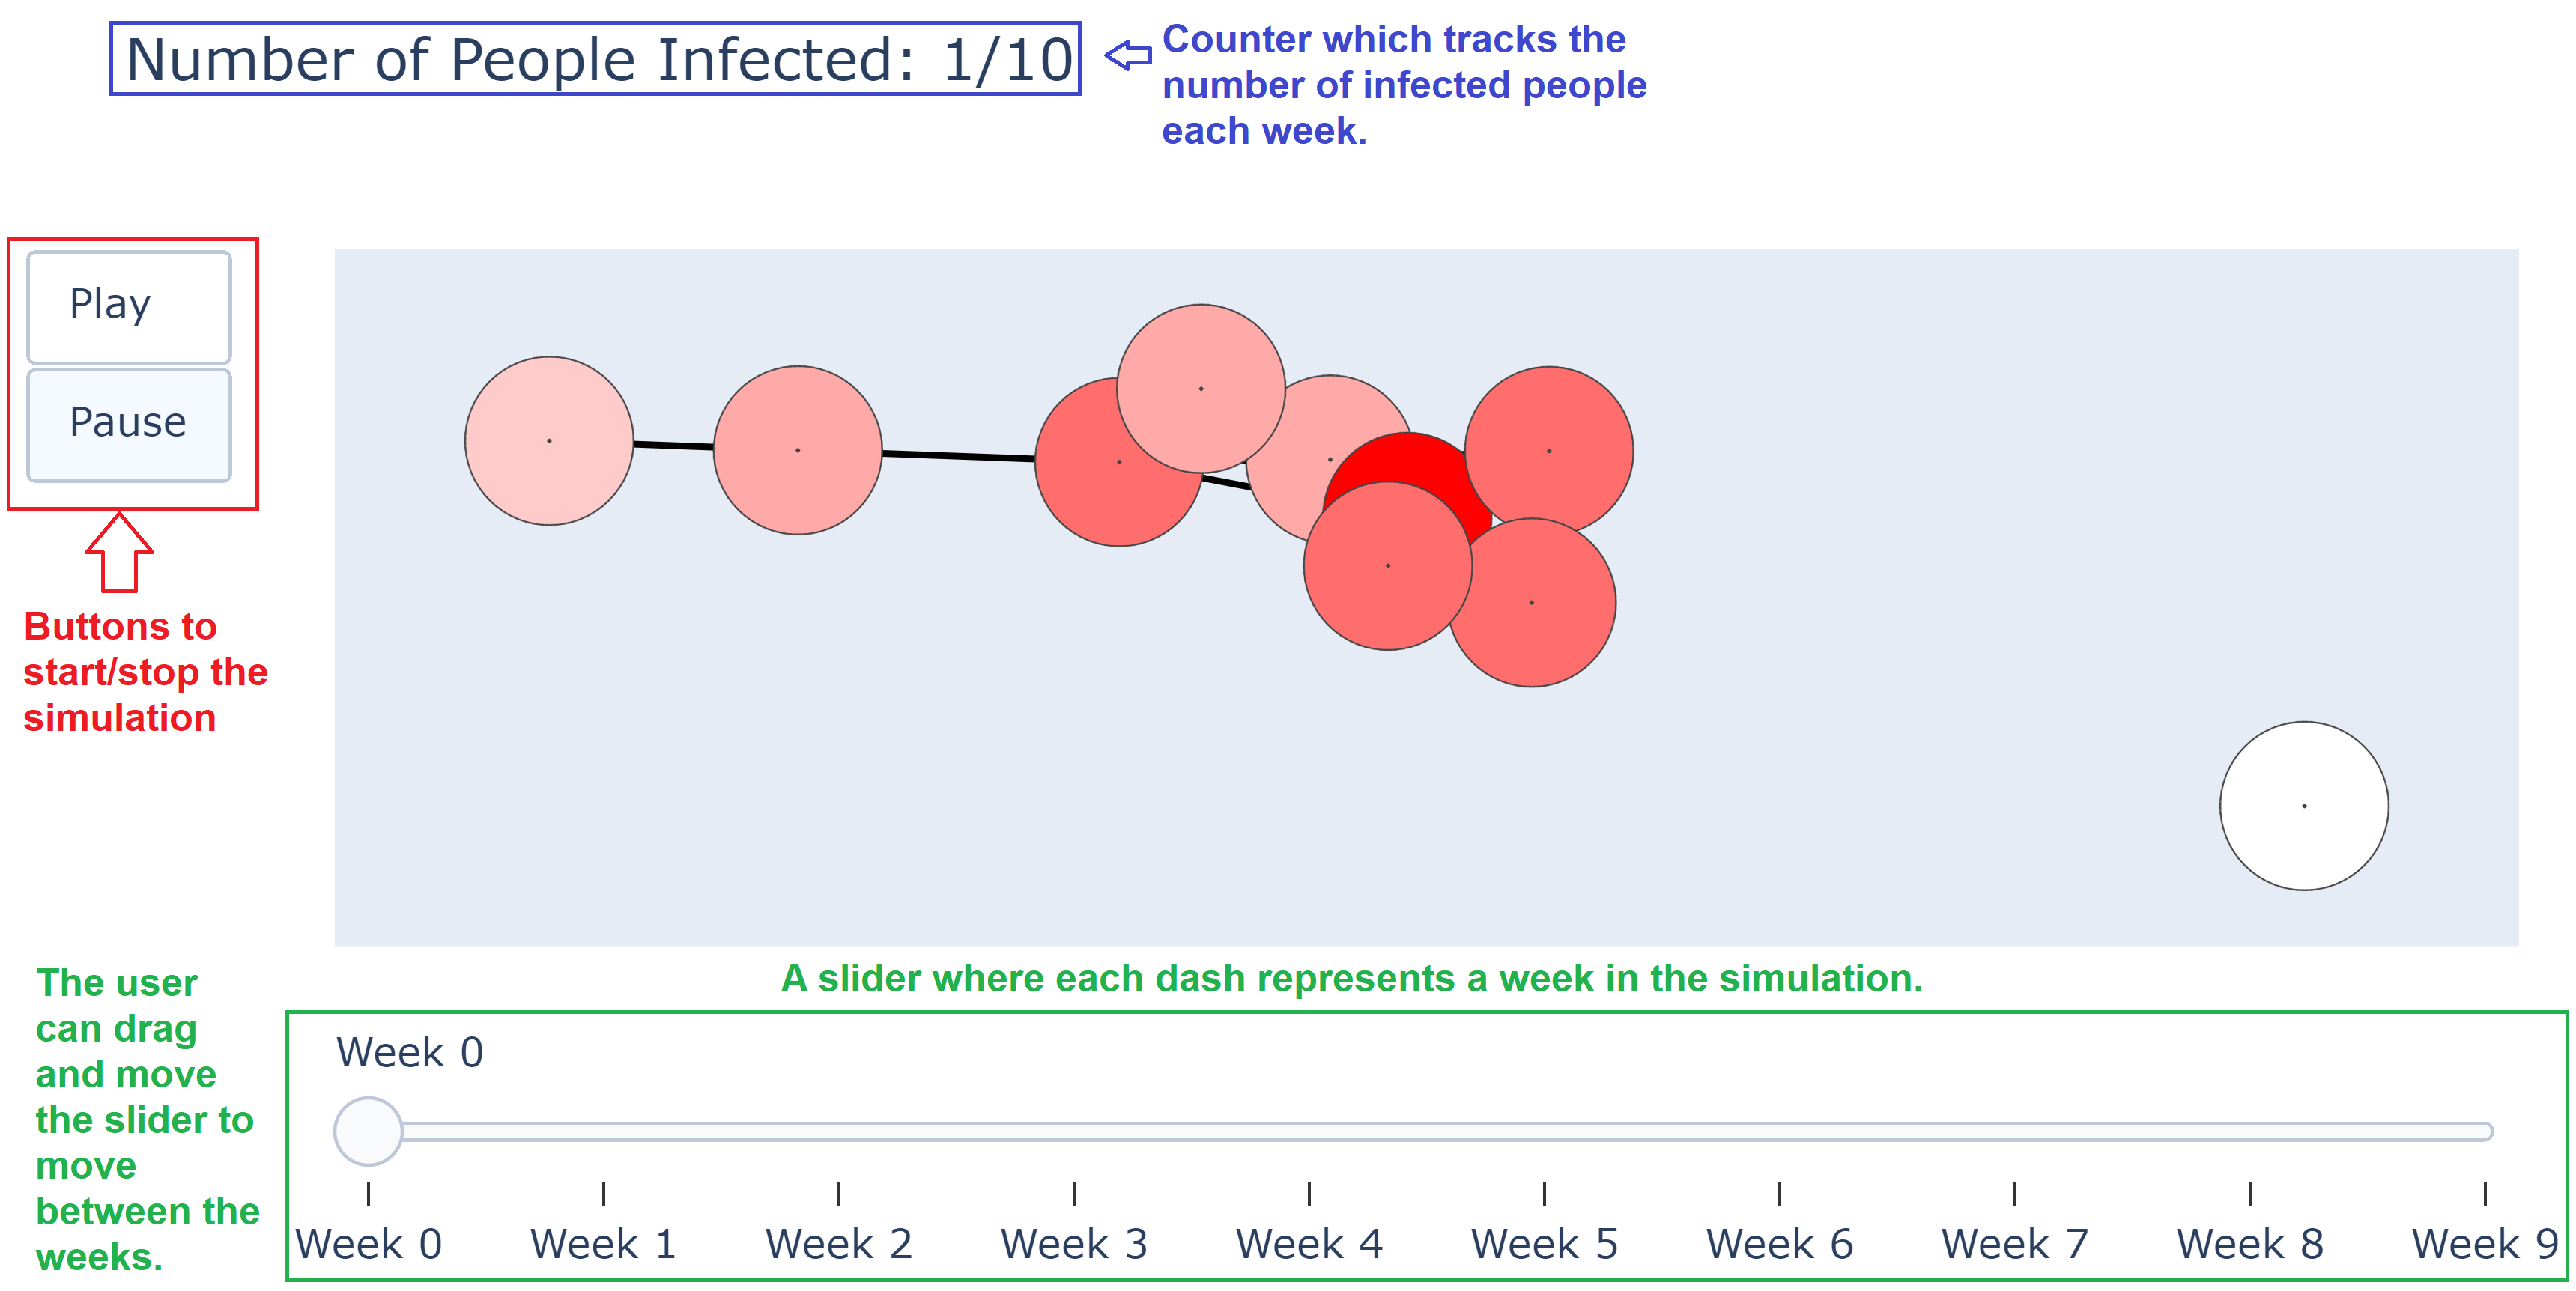
\includegraphics[width=170mm,scale=0.3]{pictures/run_csv_simulation.png}
        \caption{CSV Simulation (Zoomed for Readability)}
    \end{figure}
    \newpage
    \section*{Changes}
    The focus of our domain and focus of our project has remained the same since the project proposal, although some minor changes were once we began the implementation. We decided to use the \texttt{plotly} library instead of \texttt{matplotlib} for the visualization. This decision was made because \texttt{plotly} offers many more interactive features than \texttt{matplotlib}. This was especially important for animating the simulation. \texttt{plotly} allowed for the easy implementation of a slider and play/pause button. It provides an easy-to-use interface for the user when navigating the simulation.

    Another change was that we originally wanted to allow the user to choose which person became infected. However, upon researching into the \texttt{plotly} library, it does not have very extensive functionality for handling click events on the nodes. Furthermore, since our project focuses on how the virus spreads, instead of how it affects people on the individual level, we decided that it was okay to remove this feature of the program without compromising its functionality. We ended up choosing random nodes to infect. However, we still wanted to receive user input in this area so we let the user choose the number of nodes to infect, instead of choosing which nodes to infect.

    Finally, we originally wanted the user to be able to see a degree graph of the infected person and keep it separate from the simulation. However, once we began to implement the simulation, we realized it was feasible to merge the two aspects of the program and update the degrees of separation from an infected person dynamically as the virus spread. However, it is still possible to view the degree graph or the simulation separate from each other using the various runner functions in the main module.



    \newpage
    \section*{Discussion}
    The goal of this program was to answer the question, "How can we create an interactive visualization of the spread of COVID-19 in small communities/friend groups?" We believe that this program provides a meaningful answer to this question. By allowing the user to adjust a variety of variables in the simulation, the user is able to visualize a plethora of scenarios that model the spread of COVID-19 in real life. Let us visualize some scenarios using the program's simulation.

    In Ontario, Doug Ford's disastrous handling of the pandemic has caused vast amounts of confusion about what the lockdown rules are and as a result, more people are gathering more frequently. This can be represented in the simulation as a network with many people (60), a "high" level of contact within the network, and suppose one person is initially infected with COVID-19.
    $$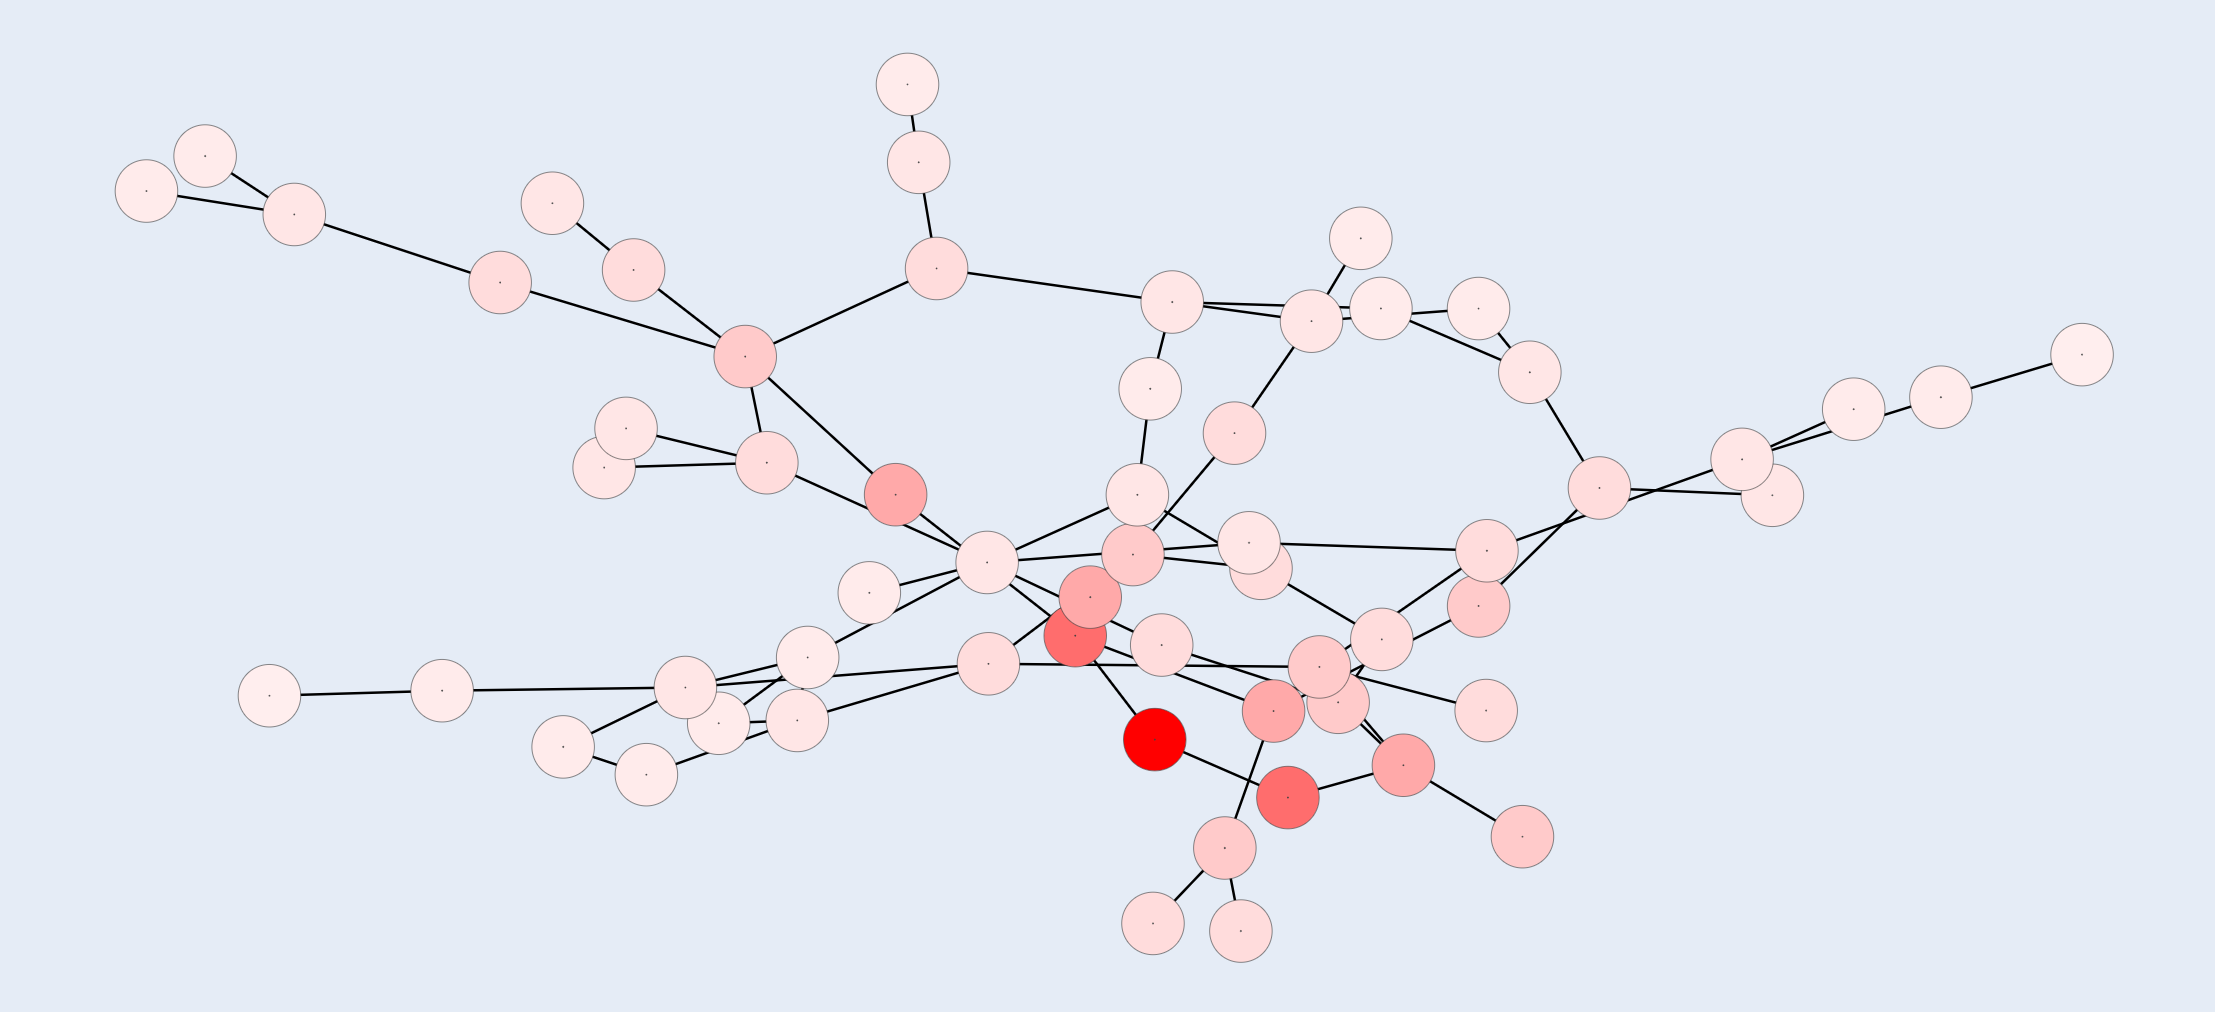
\includegraphics[scale=0.3]{pictures/week0.png}$$
    As shown in the graph above, at the very start of the simulation, the initially infected person's immediate social circle includes 2 people. In the graph below, representing 5 weeks after the initial infection, even having two neighbours causes rapid spread of the virus when the level of contact is high. At 5 weeks, half of the community (30 people) has been infected with COVID-19. Furthermore, at this stage, 20 healthy people are highly at risk of developing COVID-19 because they are neighbours to someone infected.
    $$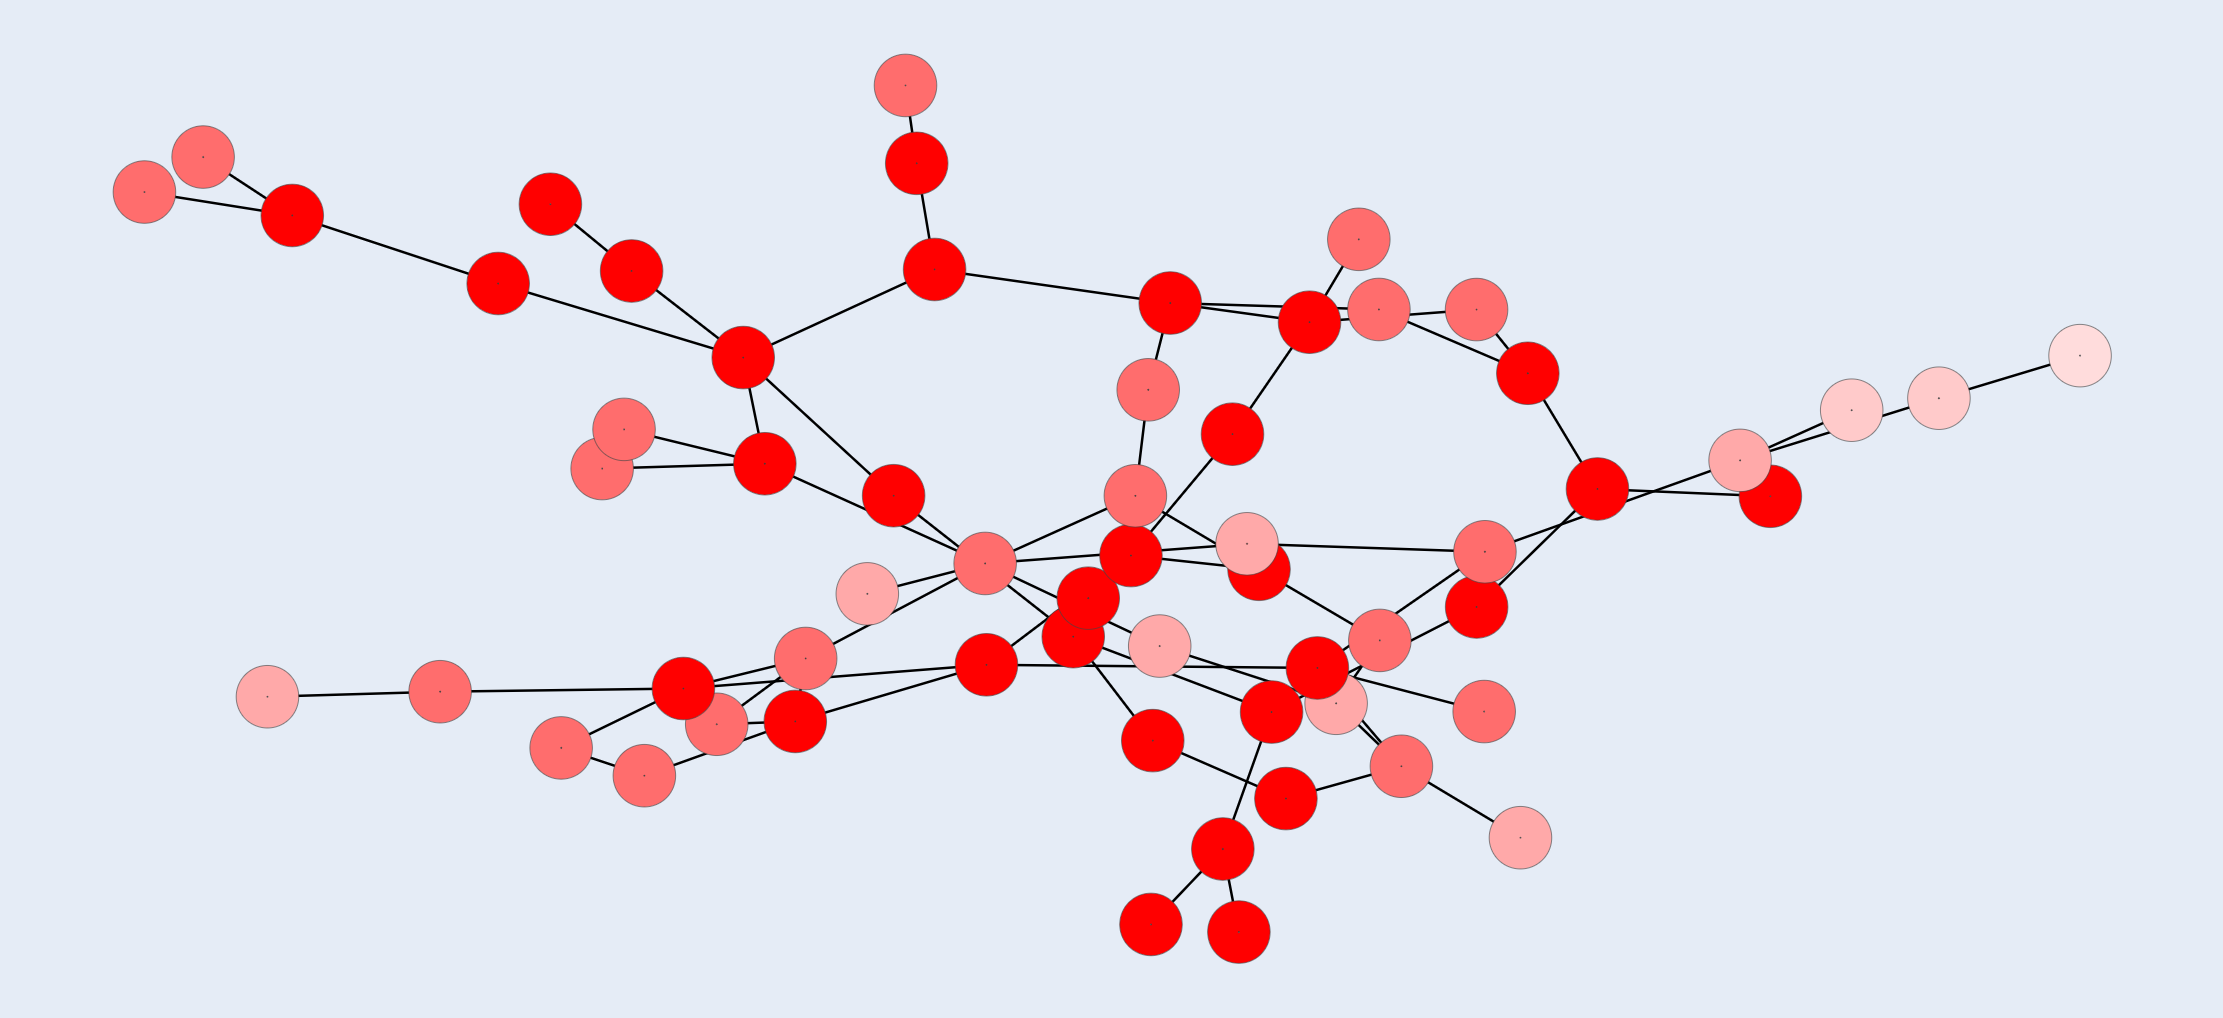
\includegraphics[scale=0.3]{pictures/week5.png}$$
    The results of this simulation show that a high number of people who are in high levels of contact with each other spreads the virus very quickly.
    In contrast, countries such as South Korea had a much more effective response to COVID-19, where a strict lockdown was imposed and social gatherings were severely restricted. Families were able to stay completely at home and keep levels of contact low. We will model this scenario with the same settings as previously, except the level of contact will be "low".
    \newpage
    \section*{Discussion Continued}
    $$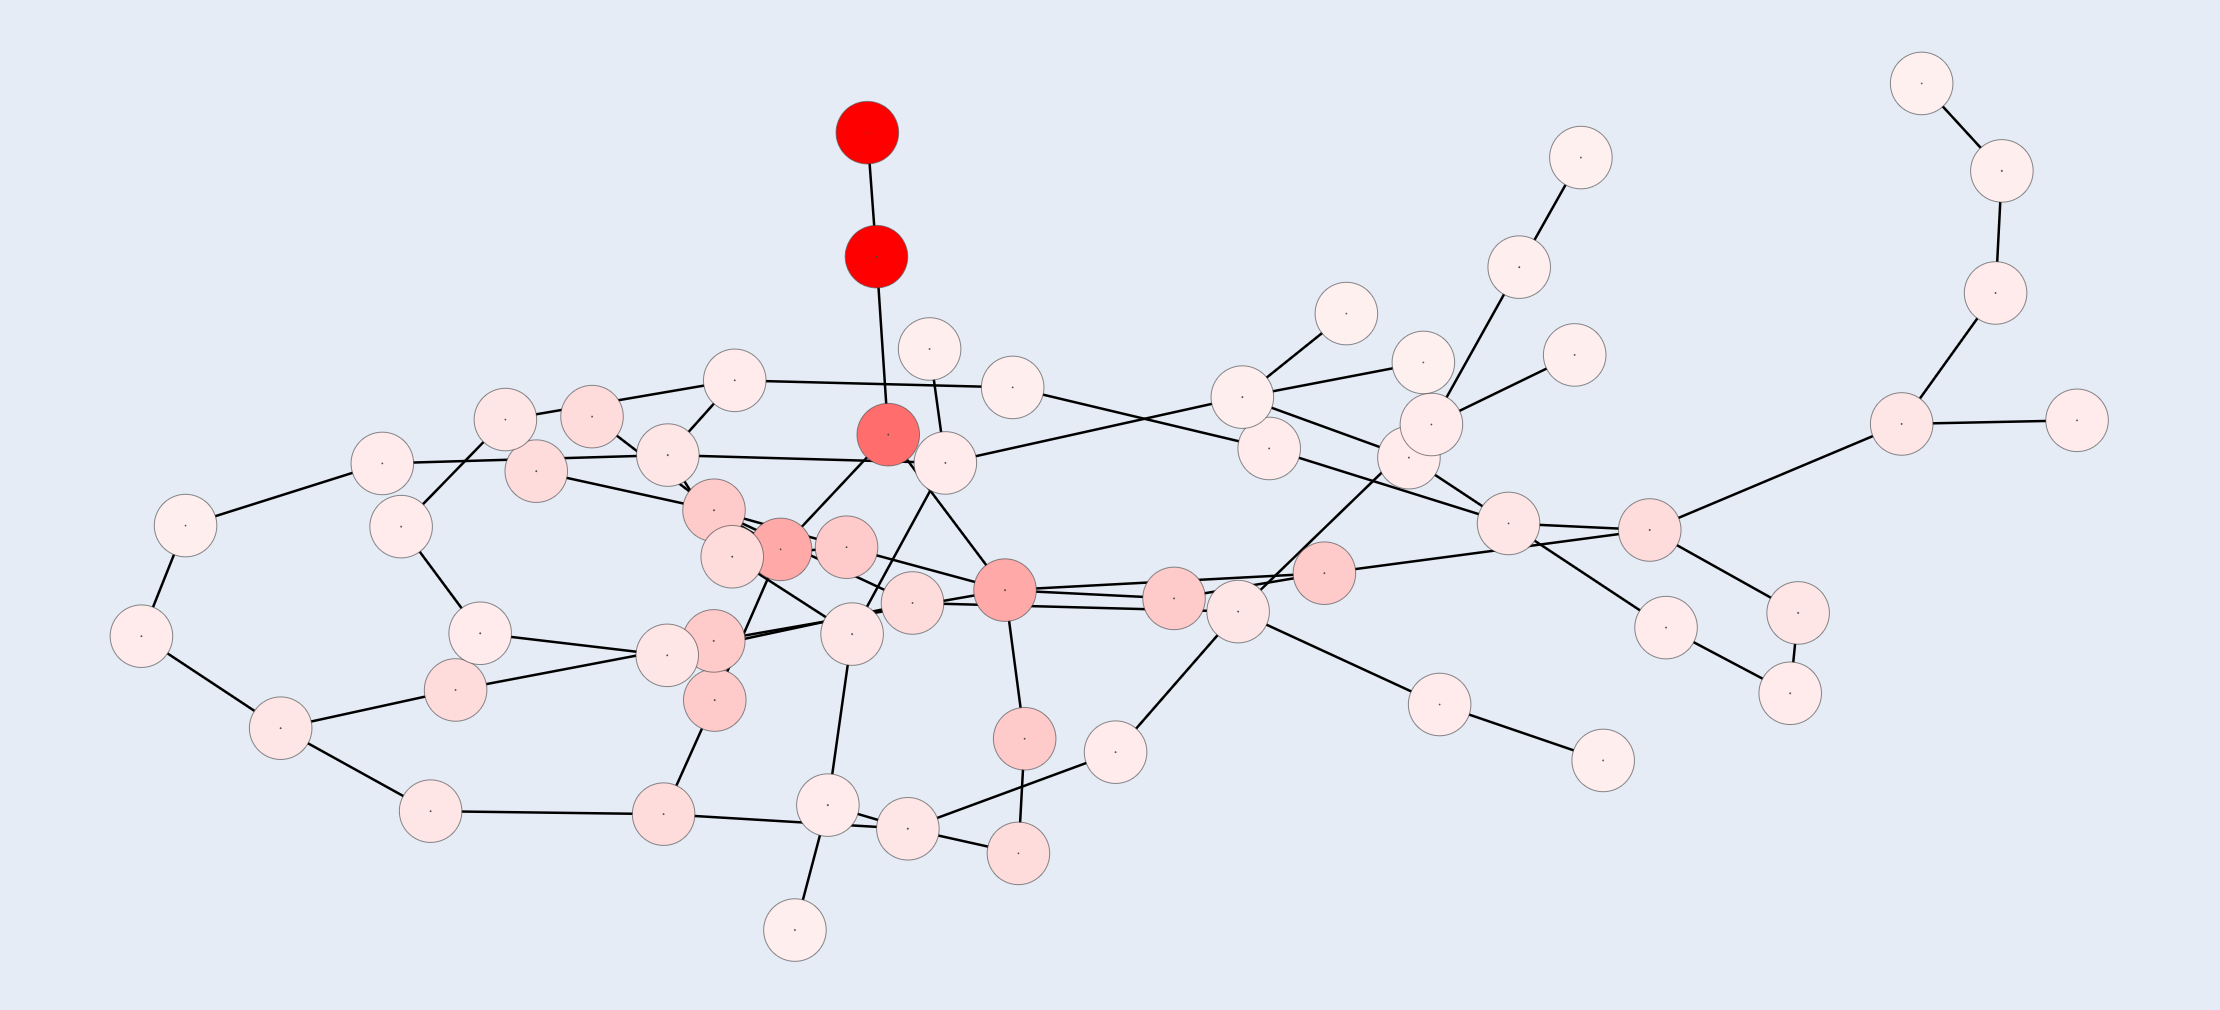
\includegraphics[scale=0.3]{pictures/week5_sk.png}$$
    The graph above is the result of a "low" level of contact after 5 weeks. Only 2 people have been infected, representing 3\% of the population. Compared to Ontario's simulation, South Korea's simulation has a 47\% lower infection rate. Furthermore, after 5 weeks, only 1 person is directly at risk of developing COVID-19 because they are neighbours with someone infected.

    Finally, consider the scenario of a retail store where the staff are connected to each other, but the customers are served remotely and do no present a considerable risk of transmitting or contracting the virus. We will represent the simulation with 30 people, a "medium" level of contact, 1 person who is initially infected, and we will make the graph disconnected. The initial setup is displayed below.

    $$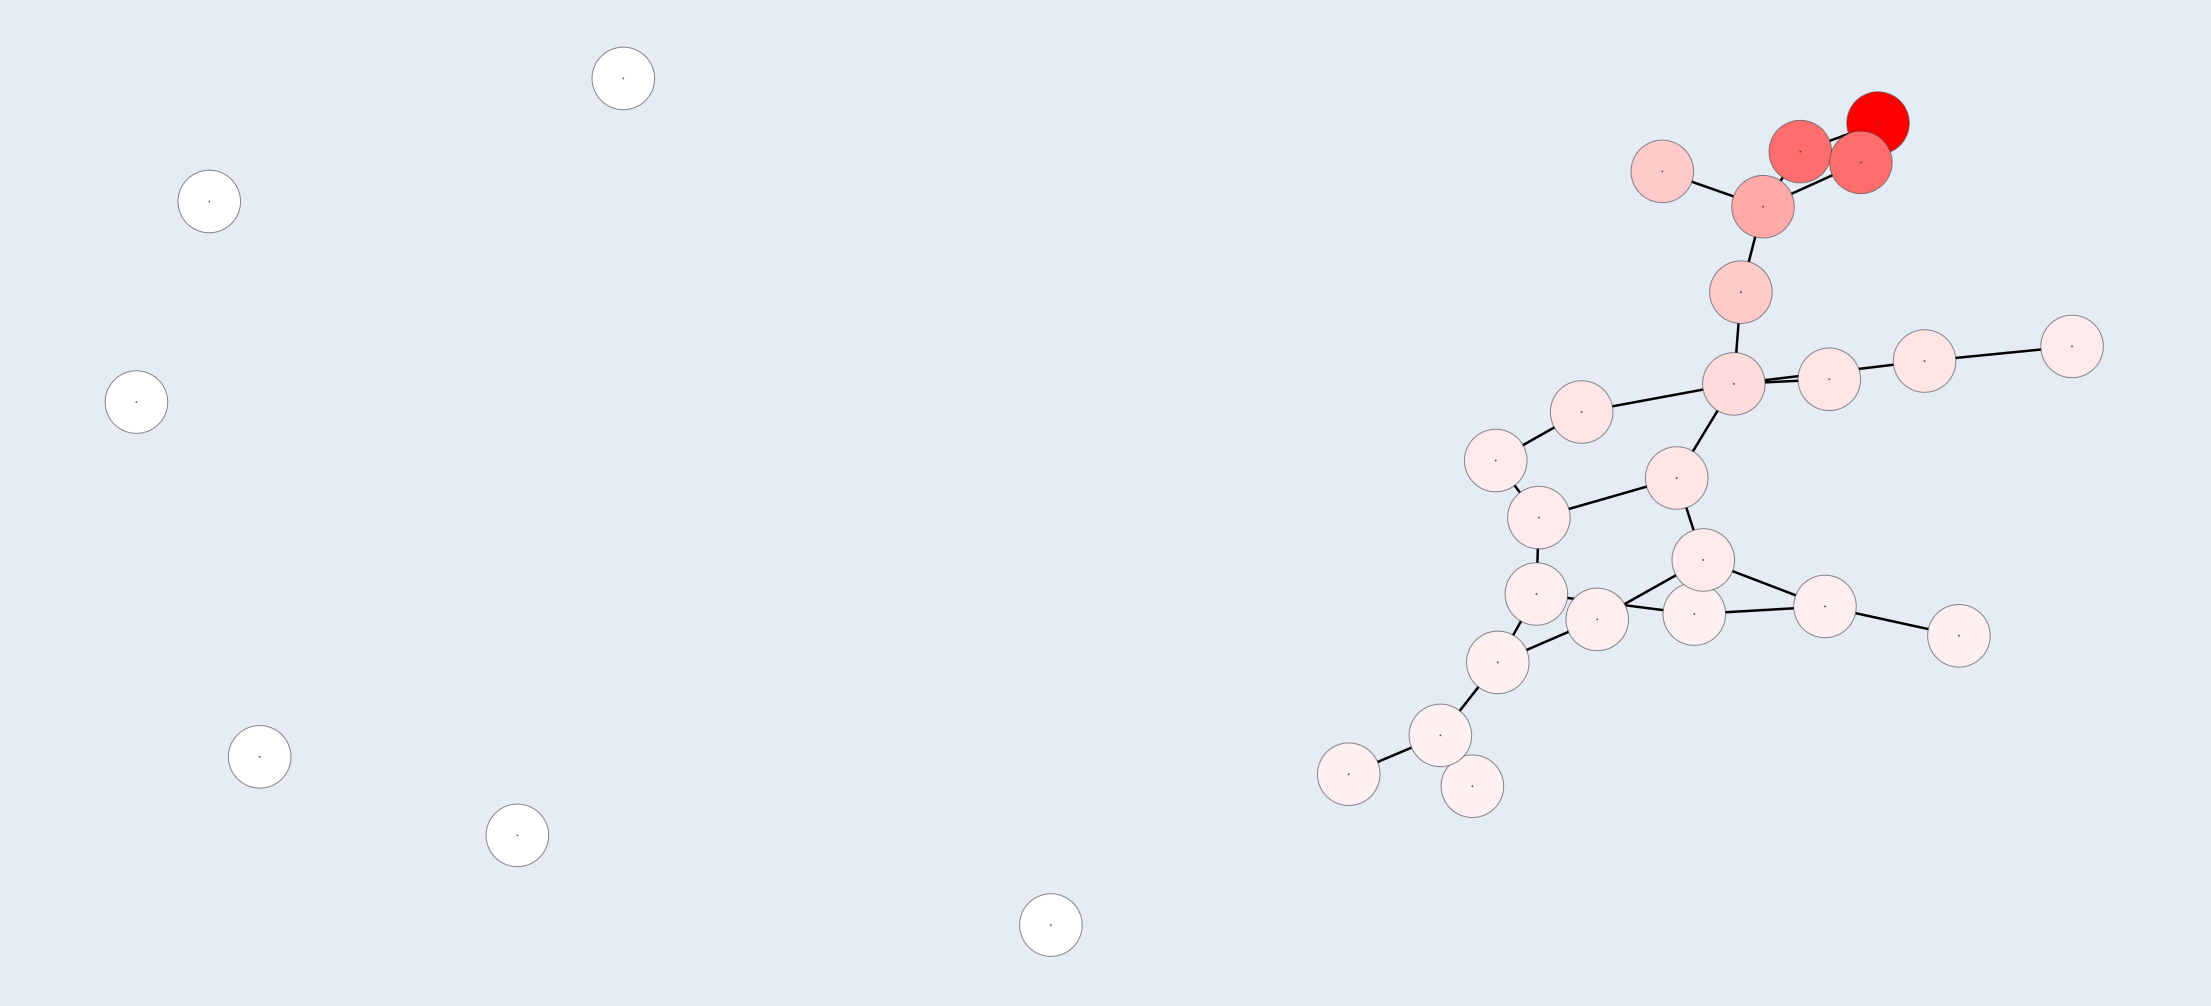
\includegraphics[scale=0.3]{pictures/disconnected_graph.png}$$
    \newpage
    \section*{Discussion Continued}
    The simulation shows that takes 17 weeks to fully infect everyone who was connected to the initially infected person (on the next page). However, all the customers who were not in contact with the staff were not infected. This scenario shows that the virus is unable to reach people who are not connected to any infected people.

    $$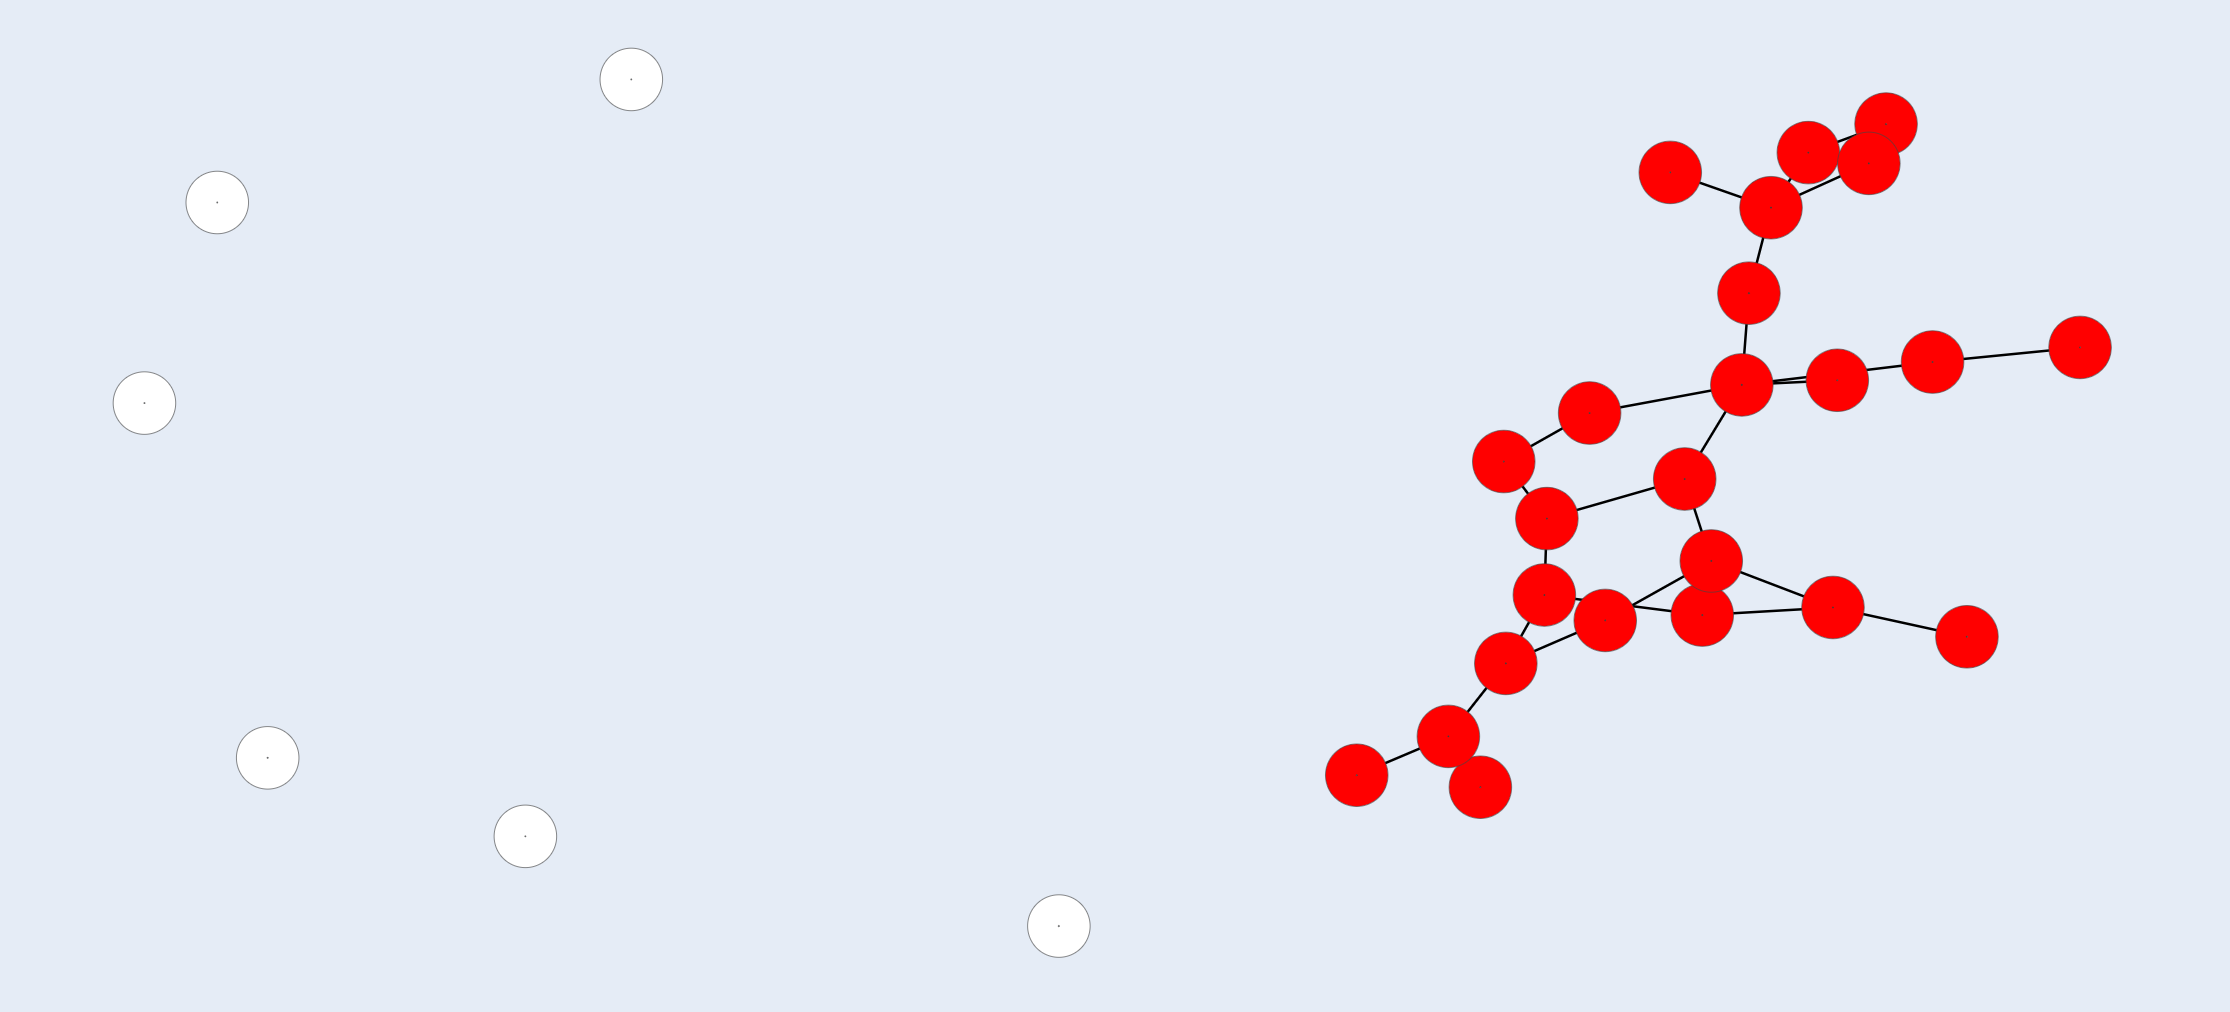
\includegraphics[scale=0.3]{pictures/fully_infected.png}$$

    These conclusions, although useful, are not surprising. However, the value of this simulation mainly lies in its ability to use a visual medium to show the user how rapidly viruses can spread. It may help the user understand why social distancing and lock downs are necessary even when the user is not infected themselves.

    A limitation that we noticed when developing the algorithm for the simulation was that it was difficult to incorporate every aspect of human behaviour that changes the spread of the virus. For example, once a community becomes a hot spot for the virus, normally, the government will shut down that area to limit transmission. This causes the number of connections and level of contact between people to decrease. Implementing this feature into the program would have been complicated, as we would have had to dynamically remove edges, change edge weights, and so on, as time progressed. Ultimately, our group decided to keep the conditions of the simulation static in order to simplify the algorithm and present an easy-to-follow visualization to the user.

    Furthermore, the program faces another limitation in that it fails to account for the different levels of severity that people who develop COVID-19 experience. Some people who develop the disease are asymptomatic, while it is fatal for others. Ultimately, we decided to prioritize showing the degrees of separation between people using a colour gradient, instead of displaying the health of the individual. Alternatively, we could have used different colours in the graph to show different levels of severity for those infected. Overall, the limitations of this program are related to the nuances of COVID-19 and human behaviour that are difficult to capture in a simulation.

    A further expansion of this program would involve solving some of the limitations in this program that were brought up. Namely, improving the simulation to better resemble real life. A good way to do this would be to use the different levels of severity one can experience with COVID-19 and group the patients into categories similar to a SIRD model from a previous assignment. This would also contribute to a more robust visualization because the user could see how COVID-19 affects people and communities differently.
    \newpage
    \section*{References}
    “A Call to Action: COVID-19 Contact Tracers.” \textit{Government of Canada}, 27 Oct. 2020,\\
    \indent www.canada.ca/en/government/system/digital-government/living-digital/covid-special-articles/contact-tracers.html.
    \\ \\
    “Certain Medical Conditions and Risk for Severe COVID-19 Illness.” \textit{Centers for Disease Control and}  \\
    \indent \textit{Prevention}, Centers for Disease Control and Prevention, 22 Feb. 2021, www.cdc.gov/coronavirus/2019-
    \indent ncov/need-extra-precautions/people-with-medical-conditions.html. \\ \\
    “COVID-19 (Coronavirus): Long-Term Effects.” \textit{Mayo Clinic}, Mayo Foundation for Medical Education and \\
    \indent Research, 17 Nov. 2020, www.mayoclinic.org/diseases-conditions/coronavirus/in-depth/coronavirus-long-term-
    \indent effects/art-20490351.
    \\ \\
    “COVID-19: Why Is It Mild for Some, Deadly for Others?” \textit{Weill Cornell Medicine}, 17 Apr. 2020, \\
    \indent weillcornell.org/news/covid-19-why-is-it-mild-for-some-deadly-for-others.
    \\ \\
    Kushman, Rick. “Your Mask Cuts Own Risk by 65 Percent.”\textit{UC Davis}, 28 Oct. 2020, \\
    \indent www.ucdavis.edu/coronavirus/news/your-mask-cuts-own-risk-65-percent/.
    \\ \\
    “Reference.” \textit{Reference - NetworkX 2.5 Documentation}, 22 Aug. 2020, \\
    \indent networkx.org/documentation/stable/reference/index.html.
    \\ \\
    “Rolling Updates on Coronavirus Disease (COVID-19).” \textit{World Health Organization}, World Health Organization,
    \indent 31 July 2020, www.who.int/emergencies/diseases/novel-coronavirus-2019/events-as-they-happen.

\end{document}
